    \chapter{Methods}\label{cha:met}

    The methods utilized in this work are presented in the following chapter. Bayesian analysis and decision theory are introduced. Focus is laid on Bayesian inference, estimation of uncertain values and the use of loss functions in this context. These methods are incorporated in computational modeling of structural geological settings by programming in a python 3 environment. Central tools for model construction and conduction of the statistical evaluation are GeMpy and PyMC 2 in particular. These are also presented in this chapter.
    
        \section{Bayesian analysis and decision theory}
	    As implied by the name, the problems and reasoning behind decision-making are examined in the field of decision theory \citep{berger2013stat}. Such decision problems are commonly influenced by parameters that are uncertain. In statistical decision theory, available statistical knowledge is used to gain information on the nature of these uncertainties. (Such uncertain parameters can be considered as numerical quantities.) In order to find the best decision to a problem, it is possible to combine sample information with other aspects such as the possible consequences of decision-making and the availability of prior information on our uncertainties. Decision consequences are expressed as gains in economic decision theory and as losses, which equal negative gains, in statistics. Prior information might be given for example based on experience from previous similar problems or from expert knowledge (see Batvold and Begg). The approach of utilizing priors is known as Bayesian analysis, which is explained in the following \citep{berger2013stat}. (It goes well with decision theory.)
	    
	    \subsection{Basic elements}
	    First, some basic elements are to be defined. The unknown (uncertain) quantity influencing decision-making is usually denominated as the state of nature $\theta$ \citep{berger2013stat}. Given statistical information on $\theta$ in the form of probability distributions, $\theta$ is called the parameter. 
	    Decisions are also referred to as actions $a$.
	    The outcome of statistical tests in form of information or statistical evidence is denoted as $X$.	    
	    Loss is defined as $L(\theta,a)$, so $L(\theta_1,a_1)$ is the actual loss incurred when action $a_1$ is taken while the true state of nature is $\theta_1$ \citep{berger2013stat}. Loss, expected loss and loss functions are explained in detail further below.  
        
        \subsection{Bayesian inference}
        Bayesian inference is most importantly characterized by its preservation of uncertainty, in contrast to standard statistical inference \citep{davidson2015}. Probability is seen as a measure of belief for an event to occur. It has been argued by \cite{davidson2015}  that this Bayesian approach is intuitive and inherent in the natural human perspective. These beliefs can be assigned to individuals \citep{davidson2015}. Thus, different and even contradicting beliefs about the probability of an event might be held by different individuals, based on variations and disparities in the information available to each one individual \citep{davidson2015}.
        
        The initial belief or guess about an event A can be denoted as P(A) \citep{davidson2015}. This is used as the so-called prior probability on which Bayesian updating is based. The beliefs about the occurrence of an event are revalued in the presence of additional information, i.e. the observation of new evidence X. These observations are included as likelihoods P(X$|$A). This process of updating results in a posterior probability P(A$|$X) \citep{davidson2015}. It is important to note that the prior is not simply discarded but re-weighted by Bayesian updating. It was also pointed out by \citet{davidson2015} that by utilizing an uncertain prior, the potential for wrongfulness of the initial guess is already included. This means that Bayesian updating is about reducing uncertainty in a belief and reaching a guess that is less wrong \citep{davidson2015}.
        Bayesian updating is defined by and conducted via the following equation, called the Bayes' Theorem:
        
        \begin{equation}\label{eq:BayesTheorem}
        P(A|X) = \frac{P(X|A)P(A)}{P(X)}
        \propto P(X|A)P(A)
        \end{equation}
     
        -Law of Large Numbers!
                
        \subsection{Estimation}
        The resulting posterior distribution can be used to acquire point estimates for the true state of nature $\theta$. Common and simple examples for such estimators are the mode (i.e. the generalized maximum likelihood estimate), the mean and the median of a distribution \citep{berger2013stat}. The presentation of a point estimate should usually come with a measure for its estimation error. According to \citet{berger2013stat}, the posterior variance is most commonly used as an indication for estimate accuracy. However, it is argued by \citet{davidson2015} that by using pure accuracy metrics, while this technique is objective, it ignores the original intention of conducting the statistical inference in cases, in which payoffs of decisions are valued more than their accuracies. A more appropriate approach can be seen in the introduction of loss and the use of loss functions \citep{davidson2015}.
        
        \subsection{Expected loss and loss functions}\label{sec:loss} 
        Loss is a statistical measure of how bad an estimate is, i.e. how much is lost by making a certain decision. Gains are considered by statisticians as negative losses \citep{davidson2015}.
        The magnitude of an estimate's loss is defined by a loss function, which is a function of the estimate of the parameter and the true value of the parameter \citep{davidson2015}:
        
        \begin{equation}\label{eq:LossFunction}
        L(\theta,\hat{\theta}) = f(\theta,\hat{\theta})
        \end{equation}
        
        So, "how bad" a current estimate is, depends on the way a loss function weighs accuracy errors and returns respective losses. Two standard loss functions are the absolute-error and the squared-error loss function. Both are simple to understand and commonly used \citep{davidson2015}.
        
        As implied by its name, the absolute-error loss function returns loss as the absolute error, i.e. the difference between the estimate and the true parameter \citep{davidson2015}:
        
        \begin{equation}\label{eq:AbsLossFunction}
        L(\theta,\hat{\theta}) = |\theta - \hat{\theta}|
        \end{equation}        
        
        Accordingly, losses increasing linearly with the distance to the true value are returned for respective estimates. This means that all differences between relative errors are weighed equally, no matter whether they are found in the realm of relatively small or relatively large errors \citep{hennig2007}.
        
        Using the squared-error loss function returns losses that increase quadratically with distance of the estimator to the true parameter value \citep{davidson2015}:
        
        \begin{equation}\label{eq:SqrLossFunction}
        L(\theta,\hat{\theta}) = |\theta - \hat{\theta}|^2
        \end{equation}        
        
        This exponential growth of loss also means that large errors are weighed much stronger than small errors. This might come with over-valuation of distant outliers and misrepresentation of magnitudes in distance. Regarding this, the absolute-error loss function can be seen as more robust \citep{davidson2015}.\\
        Both of these standard loss functions are symmetric and can be described as objectively aiming at a high precision in estimating the true parameter value.
        \citet{davidson2015} and \citet{hennig2007} propose that it might be useful to move away from these type of objective loss functions to the design of customized loss functions that specifically reflect an individual's (i.e. the decision maker's) objectives, preferences and outcomes. \citet{hennig2007} argue that choosing and designing a loss function involves the translation of informal aims and interests into mathematical terms. This process naturally implies the integration of subjective decisions and subjective elements. According to \citet{hennig2007}, this is not necessarily unfavorable or "less objective", as it may better reflect an expert's perspective on the situation and contribute to a productive scientific discussion.\\        
        The standard loss functions defined above are symmetric, but can easily be adapted to be asymmetric, for example by weighing errors on the negative side stronger than those on the positive side. Preference over estimates larger than the true value (i.e. overestimation) is thus incorporated in an uncomplicated way \citep{davidson2015, hennig2007}. Much more complicated designs of loss functions are possible, depending on purpose, objective and application \citep{davidson2015}. Some case-specific loss functions are designed in the following chapters of this work. \\
        The presence of uncertainty during decision making implies that the true parameter is unknown and thus the truly incurred loss $L(\theta,a)$ cannot be known at the time of making the decision \citep{berger2013stat, davidson2015}. The Bayesian perspective considers unknown parameters as random variables and samples that are drawn from the posterior distribution as possible realizations of the unknown parameter, i.e. all possible true values are represented by this distribution \citep{davidson2015}. A suitable alternative to the actual loss is to consider a decision's expected loss and to make a decision that is optimal in relation to this expected loss \citep{berger2013stat}. \\        
        Given a posterior distribution $P(\theta|X)$, the expected loss of choosing an estimate $\hat{\theta}$ over the true parameter $\theta$ (after evidence X has been observed) is defined by the function below \citep{davidson2015}:
        
        \begin{equation}\label{eq:ExpectedLoss}
        l(\hat{\theta}) = E_{\theta}[L(\theta,\hat{\theta})]
        \end{equation}  
        
        The expectation symbol $E$ is subscripted with $\theta$, by which it is indicated that $\theta$ is the respective unknown variable. This expected loss as defined above, is also referred to as the risk of estimate $\hat{\theta}$ \citep{davidson2015}.
        
        By the Law of Large Numbers, the expected loss of $\hat{\theta}$ can be approximated drawing a large sample size $N$ from the posterior distribution, respectively applying a loss function $L$ and averaging of the number of samples \citep{davidson2015}:
        
        \begin{equation}\label{eq:ExpectedLoss2}
        \frac{1}{N}\sum_{i=1}^{N} L(\theta_i,\hat{\theta}) \approx E_{\theta}[L(\theta,\hat{\theta})] = l(\hat{\theta})
        \end{equation}
        
        Minimization of a loss function returns a Bayesian point estimate known as Bayes action $\delta^P(X)$, which is the estimate, action or decision with the least expected loss according to the loss function \citep{berger2013stat}. For a unimodal and symmetric absolute-error loss function, the Bayes action is simply the median of the posterior distribution, while squared-error loss it is the mean \citep{davidson2015, berger2013stat}. The MAP (maximum a posteriori) estimate is the minimizing solution for the posterior using zero-one loss \citep{davidson2015}. The possibility of more than on minimum also implies that several Bayes actions can exist for one problem \citep{berger2013stat}.\\
        \citet{davidson2015} implemented different risk affinities by simply  introducing a risk parameter into the loss function. By using different values for this parameter, it can be represented how comfortable an individual is with being wrong and furthermore which "side of wrong" is preferred by this decision maker \citep{davidson2015}. This approach to expressing risk-affinities is used the design of loss functions in this work.
        
        %\subsection{Value of information}
        %- considering the change in gain (or loss) after regarding new information or evidence, the value of this information can be calculated
        %- in the presence of uncertainty we look at expected value of information
        %- this can be used as a measure, to assess if the effort to attain new evidence or information is worth it
        %- also as a measure to see how much additional information is worth to different actors with different risk affinities
        %- here we use the comparison between Bayes actions before and after Bayesian updating
        
        \section{Application in structural geological modeling}
        In this work, these methods of Bayesian analysis and decision theory are applied in the field of geological structural modeling. The fundamental approach follows closely the research conducted by \citet{delaVarga2016} and builds upon their findings.\\
        According to them, structural geological modeling can be regarded as a forward problem and the elements of Bayesian inference can be specified in this context as follows:
        \begin{enumerate}
        	\item \textbf{Mathematical forward model ($M$)}: The connections between parameters $\theta$ and observed data $y$ are defined in this mathematical model. ...
        	\item \textbf{Model parameters ($\theta$)}: These model-defining parameters, such as the position or dip of layers and faults in geological settings, can be deterministic or stochastic. In the latter case, they are uncertain parameters to which a probability distribution is assigned.
        	\item \textbf{Observed data ($y$)}: This is any type of additional information that can be related to the forward modeling results and might possibly be used to reduce uncertainty. Such data can be gained by measurements and observations, for example by core sampling, well-log analysis or seismic acquisition. 
        	\item \textbf{Likelihood functions ($p(y|\theta)$}: Links between the previous parameters $\theta$ and the additional data $y$ are established by these functions in way that they reflect the likelihood of the parameter states given the observations \citep{delaVarga2016}.
        \end{enumerate}
        
        A fundamental sequence of the inference process was proposed by \citet{gelman2014bayesian}, adapted by \citet{delaVarga2016} and is subsequently adjusted for the application in this work as follows:
        \begin{enumerate}
        	\item \textbf{Setting up a full probability model}: A multi-dimensional joint probability space is to be generated, taking into account the probability distributions of every model parameter $\theta$. (- here, this not only results in the creation of geological models, but is subsequently also coupled with algorithms which deduct economic realizations from these models.)
        	\item \textbf{Conditioning on observed data}: Subsequently, an appropriate posterior distribution $p(\theta|y)$ is to be calculated by conditioning the parameters $\theta$ on the observed data $y$ given the likelihood $p(\theta|y)$. This is the step of Bayesian updating of the belief about the parameter uncertainty given new information.
        	In a chosen model ($M$), this is achieved by linking parameters and data through deterministic operations which are additionally compared to the likelihood functions. It is pointed out by \citet{delaVarga2016} that any combination of parameter-observation connections is allowed, i.e. not all parameters need to be necessarily connected to all observed data. After all conditional probabilities have been set up, the Bayes Theorem (Equation \ref{eq:BayesTheorem}) is applied to attain the posterior. However, due to the multi-dimensionality given in geological problems, the use of Markov chain Monte Carlo methods is advised to achieve this as described in Section \ref{sec:mcmc} below.
        	\item \textbf{Evaluation of the posterior model}: Depending on the aim of the study, a post-processing analysis can be conducted accordingly. \citet{delaVarga2016} focused on the examination of the posterior distributions of the parameters $\theta$ and the generated models, particularly regarding information entropy within the model space. In this work, the geological models are assigned an economic meaning by declaring them potential petroleum reservoirs and introducing customized loss functions to reflect the economic interest of decision makers in developing respective resource extraction projects (see Section \ref{sec:loss}). Shifts in Bayes actions are considered a measure for the influence of Bayesian inference on decision-making and the significance of additional observations for different decision makers.
        \end{enumerate}
        
        \subsection{Markov chain Monte Carlo sampling (MCMC)}\label{sec:mcmc}
        Despite the apparent simplicity of the Bayes Theorem, a direct analytical calculation and exact inference of the posterior distribution P(A$|$X) is rarely possible in non-idealized cases, due to intractability in multi-dimensional spaces \citep{hoffman2014no, delaVarga2016}. Thereby arises the necessity to resort to methods of statistical inference approximation. Markov chain Monte Carlo (MCMC) sampling has proven to be a generally applicable and reliable method for exploring multi-dimensional parameter spaces in an intelligent way \citep{hoffman2014no, davidson2015}. \citet{gilks2005markov} has emphasized the significance of MCMC for the application of Bayesian statistics.
        %In Monte Carlo integration, random samples are drawn from a target distribution, such as our posterior distribution P(A$|$X), to approximate the integral or probability density function in terms of an expectation:
        
        %\begin{equation}\label{eq:MonteCarlo}
        %        E[P(A|X)] \approx \frac{1}{N}\sum_{n=1}^{N}P(A|X)
        %\end{equation}
        In the ordinary Monte Carlo approach, random independent samples are drawn from a target distribution in order to approximate its shape \citep{gilks2005markov, delaVarga2016}. High-dimensional parameter spaces as found in Bayesian applications lead to complex shapes and often make independent sampling infeasible \citep{gilks2005markov}. This can be solved by extending the Monte Carlo principle with a Markov chain, in which every sample iteration of the parameter $\theta^{(t+1)}$ is dependent uniquely on the previous value $\theta^{(t)}$ \citep{gilks2005markov, delaVarga2016}.\\
        The general principle of MCMC can be described as follows: 
        Drawing representative samples from an target distribution of unknown shape is based on the conduction of a so-called random walk on the parameter distribution space. T sampling steps are to be performed. The first sampling location is chosen at random. With each subsequent step, a new sampling location is proposed. The new sample value is then related to the previous step. According to a weight defined by the scaled up candidate density of the value, the proposed step is then accepted or rejected. In the case of acceptance, the value is added to the sample trace and the process is continued from the current location. In the case of rejection, sampling is reverted to the previous accepted step \citep{schaaf2017, delaVarga2016}. The intention behind this concept it to achieve convergence of the sampling algorithm towards areas of high probability \citep{davidson2015}.\\ Variations in the way of how new  sample steps are proposed and in the acceptance-rejection condition result in different single MCMC sampling methods \citep{schaaf2017, delaVarga2016}. Various algorithms for random MCMC walks have been developed for over more than six decades and advancements have still been made in recent years. Common examples for such algorithms are the Metropolis-Hastings samplers as devised by \citet{metropolis1953equation} and generalized by \citet{hastings1970}. The Gibbs sampler \citep{geman1984stochastic} is another well-known method. 
        For the purspose of this work, an adaptive Metropolis-Hastings sampler is used.\\
        In Metropolis-Hastings methods, each sampling step at iteration t is determined by a candidate probability distribution $q(\theta,\theta^{'})$, from which a proposed sample $\theta^{'}$ is drawn \citep{delaVarga2016}. The acceptance-rejection condition is defined by the acceptance ratio $a(\theta^{'},\theta)$:
        
        \begin{equation}\label{eq:acceptance_ratio}
        a(\theta^{'},\theta)=\frac{p(\theta^{'})p(y|\theta^{'})}{p(\theta)p(y|\theta)}
        \end{equation}
        
        To ensure a thorough exploration of the probability space, the transition to higher probability densities should not be enforced in every case but selectively. This is assured by relating the acceptance ratio from Equation \ref{eq:acceptance_ratio} to a random value $u$ from a Uniform distribution $U(0,1)$ as follows:
        
        \begin{equation}\label{eq:transition_selectivity}
        \theta^{(t+1)}=\begin{cases}
        \theta^{'} & $if $ a(\theta^{'},\theta)>U(0,1)\\
        \theta^{t} & $otherwise$\\
        \end{cases}
        \end{equation}
        
        Thereby, the algorithm assigns high probabilities to high-density points and low probabilities to low-density points, so that the chain state is moved accordingly \citep{delaVarga2016}.\\
        Metropolis methods are furthermore defined by the step size scale factor that is chosen. While large steps are good for exploration of the space and mixture in the chain, acceptance rates are low. Small steps have better acceptance rates, but lead to slower exploration and convergence of the algorithm \citep{delaVarga2016}.\\
        The Adaptive Metropolis (AM) by \citet{haario2001adaptive} is used in this work. It adapts the traditional Metropolis-Hastings by incorporating the ability of continuous step size tuning during convergence, by taking into account the full information saved along the process. This is achieved by generating a covariance matrix that is updated every iteration. The adaptive nature of the process enables fast convergence for non-linear distributions while maintaining ergodicity \citet{haario2001adaptive, delaVarga2016}. Its suitability for multi-dimensional distribution spaces make it an excellent method for dealing with complex models such as the structural geological models in this work \citep{schaaf2017}     
        
        \subsection{Structural geological forward modeling}\label{sec:struc_geo_modeling}       
        Performing forward modeling in the context of structural geology requires the use of a suitable modeling step. Additionally, for the application in a probabilistic setting, the method should enable fully automatic reconstruction of the model, when parameters are changed. The application in this work follows the example of \citet{delaVarga2016} and relies on the use of implicit interpolation for geological modeling, a method developed and elaborated by \citet{Lajaunie1997} and \citet{calcagno2008geological}.\\
        This implicit method relies on the interpolation of a potential field scalar function $T(\vec{x})$ of any point $\vec{(x)}$ in a 3D space, and thus reflects the geometry of geological structures \citep{calcagno2008geological}. Modeling $T(\vec{x}$ is achieved by cokriging that regards two forms of data: (i) contact points on geological interfaces through increments of the potential field $T(\vec{x})-T(\vec{x}^{\,'})$ and (ii) orientation data as gradients, i.e. partial derivatives of the potential field $\delta T(\vec{x})/\delta u_\beta$ in each directon $u$ \citep{calcagno2008geological}. The respective estimator is defined as follows:
        \begin{equation}\label{eq:Cokriging_Estimator}
                T(\vec{x})-T(\vec{x_0})=\sum_{\alpha=1}^{M}\mu_\alpha(T\vec{x_\alpha}-T(\vec{x}^{\,'}_\alpha))+\sum_{\beta=1}^{N}\nu_\beta\frac{\delta T}{\delta u_\beta}(\vec{x}_\beta),
        \end{equation}
        
        where $\vec{x_0}$ is an arbitrary origin, $M$ and $N$ are the total number of data points and partial derivatives respectively, and their relative contributions are weighed by the factors $\mu_\alpha$ and $\nu_\beta$. Furthermore, $T$ is assumed to be a random function defined by polynomial drift and a stationary covariance $K(h)$ \citep{calcagno2008geological}. The use of a cubic covariance model is suggested by \citet{calcagno2008geological}, based on the results from studies conducted by \citet{aug2004modelisation} and \citet{chiles2004modelling}.\\
		\begin{figure}[h]
			\centering
			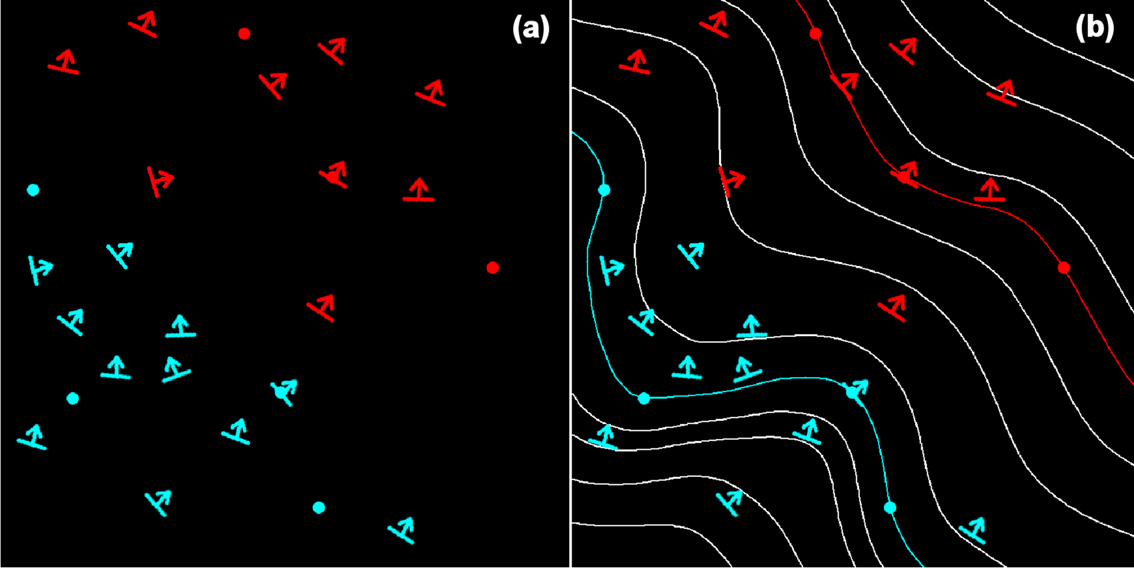
\includegraphics[width=1\textwidth]{Figures/calcagno_pot_field.png}
			\caption{woo a potential field! from \citet{calcagno2008geological}}\label{fig:pot_field}
		\end{figure}        
        Resulting potential fields can be used to describe geological interfaces as iso-surfaces in any kind of 3D geometry \citep{calcagno2008geological}. Fault geometries can be interpolated analogously. These can be infinite in the 3D space, interrelated in a fault network or finite. To account for the effect of faults on geological layers, discontinuous potential fields are created by applying discontinuous drift functions in the cokriging system. Additionally, geological rules allow for the representation of several types of interactions between sets of geological layers \citep{calcagno2008geological}.\\
        It is pointed out by \citet{calcagno2008geological}, that this method is particularly appropriate for cases in which knowledge about the geology is only given a sparse locations and is thus applicable for a wide variety of typical problem in geological settings. Its suitability for this work is furthermore emphasized by the possibility to modify the topology-defining geological pile to achieve different geometric realizations without altering the data. The model can thus be updated in the face of new data or interpretations \citep{calcagno2008geological}.
        
		\subsection{Implementing Bayesian analysis numerically with Python and PyMC}
		Bayesian analysis can be conducted using probabilistic programming \citep{salvatier2016pymc3}. For doings this, the programming language of choice in this work is Python. The merits of Python have been pointed out by \citet{behnel2010, salvatier2016pymc3, Langtangen2008}. Development is facilitated by an expressive but concise and clean syntax that is easy to learn. Python is dynamic, compatible with multiple platforms and offers good support for numerical computing. Integration of other scientific libraries and extension via C, C++, Fortran or Cython is easily possible \citep{behnel2010, salvatier2016pymc3, Langtangen2008}. Python is thus a straightforward tool for the implementation of central components of Bayesian analysis, such as custom statistical distributions and samplers \citep{salvatier2016pymc3}. 
		
		In probabilistic programming, programming variables are used as components to build probabilistic models \citep{davidson2015}. 
		
		The numerical implementation of Bayesian analysis is further aided by the use of the Python library PyMC3, which was developed for conducting Bayesian inference and prediction problems in an open-source probabilistic programming framework \citep{davidson2015, salvatier2016pymc3}. Different model fitting techniques are provided in PyMC3, such as the \textit{maximum a posteriori} (MAP) method and several \textit{Monte Carlo Markov Chain} (MCMC) sampling methods \citep{salvatier2016pymc3}. 
		Name examples for state-of-the-art samplers included.
		\citet{salvatier2016pymc3} point out that the development of PyMC3 continuing, as the inclusion of further tools is planned for future updates.
		
		\subsection{Reservoir Volumetric Calculation}
		
